\documentclass[]{article}
\usepackage{lmodern}
\usepackage{amssymb,amsmath}
\usepackage{ifxetex,ifluatex}
\usepackage{fixltx2e} % provides \textsubscript
\ifnum 0\ifxetex 1\fi\ifluatex 1\fi=0 % if pdftex
  \usepackage[T1]{fontenc}
  \usepackage[utf8]{inputenc}
\else % if luatex or xelatex
  \ifxetex
    \usepackage{mathspec}
  \else
    \usepackage{fontspec}
  \fi
  \defaultfontfeatures{Ligatures=TeX,Scale=MatchLowercase}
\fi
% use upquote if available, for straight quotes in verbatim environments
\IfFileExists{upquote.sty}{\usepackage{upquote}}{}
% use microtype if available
\IfFileExists{microtype.sty}{%
\usepackage{microtype}
\UseMicrotypeSet[protrusion]{basicmath} % disable protrusion for tt fonts
}{}
\usepackage[margin=1in]{geometry}
\usepackage{hyperref}
\hypersetup{unicode=true,
            pdftitle={DNA Mismatch Distributions in R},
            pdfauthor={A.laldin},
            pdfborder={0 0 0},
            breaklinks=true}
\urlstyle{same}  % don't use monospace font for urls
\usepackage{color}
\usepackage{fancyvrb}
\newcommand{\VerbBar}{|}
\newcommand{\VERB}{\Verb[commandchars=\\\{\}]}
\DefineVerbatimEnvironment{Highlighting}{Verbatim}{commandchars=\\\{\}}
% Add ',fontsize=\small' for more characters per line
\usepackage{framed}
\definecolor{shadecolor}{RGB}{248,248,248}
\newenvironment{Shaded}{\begin{snugshade}}{\end{snugshade}}
\newcommand{\KeywordTok}[1]{\textcolor[rgb]{0.13,0.29,0.53}{\textbf{#1}}}
\newcommand{\DataTypeTok}[1]{\textcolor[rgb]{0.13,0.29,0.53}{#1}}
\newcommand{\DecValTok}[1]{\textcolor[rgb]{0.00,0.00,0.81}{#1}}
\newcommand{\BaseNTok}[1]{\textcolor[rgb]{0.00,0.00,0.81}{#1}}
\newcommand{\FloatTok}[1]{\textcolor[rgb]{0.00,0.00,0.81}{#1}}
\newcommand{\ConstantTok}[1]{\textcolor[rgb]{0.00,0.00,0.00}{#1}}
\newcommand{\CharTok}[1]{\textcolor[rgb]{0.31,0.60,0.02}{#1}}
\newcommand{\SpecialCharTok}[1]{\textcolor[rgb]{0.00,0.00,0.00}{#1}}
\newcommand{\StringTok}[1]{\textcolor[rgb]{0.31,0.60,0.02}{#1}}
\newcommand{\VerbatimStringTok}[1]{\textcolor[rgb]{0.31,0.60,0.02}{#1}}
\newcommand{\SpecialStringTok}[1]{\textcolor[rgb]{0.31,0.60,0.02}{#1}}
\newcommand{\ImportTok}[1]{#1}
\newcommand{\CommentTok}[1]{\textcolor[rgb]{0.56,0.35,0.01}{\textit{#1}}}
\newcommand{\DocumentationTok}[1]{\textcolor[rgb]{0.56,0.35,0.01}{\textbf{\textit{#1}}}}
\newcommand{\AnnotationTok}[1]{\textcolor[rgb]{0.56,0.35,0.01}{\textbf{\textit{#1}}}}
\newcommand{\CommentVarTok}[1]{\textcolor[rgb]{0.56,0.35,0.01}{\textbf{\textit{#1}}}}
\newcommand{\OtherTok}[1]{\textcolor[rgb]{0.56,0.35,0.01}{#1}}
\newcommand{\FunctionTok}[1]{\textcolor[rgb]{0.00,0.00,0.00}{#1}}
\newcommand{\VariableTok}[1]{\textcolor[rgb]{0.00,0.00,0.00}{#1}}
\newcommand{\ControlFlowTok}[1]{\textcolor[rgb]{0.13,0.29,0.53}{\textbf{#1}}}
\newcommand{\OperatorTok}[1]{\textcolor[rgb]{0.81,0.36,0.00}{\textbf{#1}}}
\newcommand{\BuiltInTok}[1]{#1}
\newcommand{\ExtensionTok}[1]{#1}
\newcommand{\PreprocessorTok}[1]{\textcolor[rgb]{0.56,0.35,0.01}{\textit{#1}}}
\newcommand{\AttributeTok}[1]{\textcolor[rgb]{0.77,0.63,0.00}{#1}}
\newcommand{\RegionMarkerTok}[1]{#1}
\newcommand{\InformationTok}[1]{\textcolor[rgb]{0.56,0.35,0.01}{\textbf{\textit{#1}}}}
\newcommand{\WarningTok}[1]{\textcolor[rgb]{0.56,0.35,0.01}{\textbf{\textit{#1}}}}
\newcommand{\AlertTok}[1]{\textcolor[rgb]{0.94,0.16,0.16}{#1}}
\newcommand{\ErrorTok}[1]{\textcolor[rgb]{0.64,0.00,0.00}{\textbf{#1}}}
\newcommand{\NormalTok}[1]{#1}
\usepackage{longtable,booktabs}
\usepackage{graphicx,grffile}
\makeatletter
\def\maxwidth{\ifdim\Gin@nat@width>\linewidth\linewidth\else\Gin@nat@width\fi}
\def\maxheight{\ifdim\Gin@nat@height>\textheight\textheight\else\Gin@nat@height\fi}
\makeatother
% Scale images if necessary, so that they will not overflow the page
% margins by default, and it is still possible to overwrite the defaults
% using explicit options in \includegraphics[width, height, ...]{}
\setkeys{Gin}{width=\maxwidth,height=\maxheight,keepaspectratio}
\IfFileExists{parskip.sty}{%
\usepackage{parskip}
}{% else
\setlength{\parindent}{0pt}
\setlength{\parskip}{6pt plus 2pt minus 1pt}
}
\setlength{\emergencystretch}{3em}  % prevent overfull lines
\providecommand{\tightlist}{%
  \setlength{\itemsep}{0pt}\setlength{\parskip}{0pt}}
\setcounter{secnumdepth}{0}
% Redefines (sub)paragraphs to behave more like sections
\ifx\paragraph\undefined\else
\let\oldparagraph\paragraph
\renewcommand{\paragraph}[1]{\oldparagraph{#1}\mbox{}}
\fi
\ifx\subparagraph\undefined\else
\let\oldsubparagraph\subparagraph
\renewcommand{\subparagraph}[1]{\oldsubparagraph{#1}\mbox{}}
\fi

%%% Use protect on footnotes to avoid problems with footnotes in titles
\let\rmarkdownfootnote\footnote%
\def\footnote{\protect\rmarkdownfootnote}

%%% Change title format to be more compact
\usepackage{titling}

% Create subtitle command for use in maketitle
\newcommand{\subtitle}[1]{
  \posttitle{
    \begin{center}\large#1\end{center}
    }
}

\setlength{\droptitle}{-2em}

  \title{DNA Mismatch Distributions in R}
    \pretitle{\vspace{\droptitle}\centering\huge}
  \posttitle{\par}
    \author{A.laldin}
    \preauthor{\centering\large\emph}
  \postauthor{\par}
      \predate{\centering\large\emph}
  \postdate{\par}
    \date{March 2019}


\begin{document}
\maketitle

\subsection{\texorpdfstring{\href{sheading-2}{Introduction and
Preface}}{Introduction and Preface}}\label{introduction-and-preface}

For all of DnaSP's wonderful functionality its visualisations leave much
to be desired. You may be tempted to use MS Excel. While Excel is
effective for many tasks it is limited in its functionality. Last time I
checked, Excel cannot handle more than 239 data points when creating a
scatter-plot and secondly, moving data from DnaSP's.out format into
Excel is tedious at best. However, this can be circumvented in a few
short steps with a little bit of code.

This tutorial is targeted towards biologists/ecologists/population
geneticists who have a very basic understanding of R but a strong
background in population genetics,( otherwise I don't know why you'd be
calculating pairwise mismatch distributions;) ).

If you already have an idea of what you are doing, feel free to download
the R script from here and use it. If you need a little bit of
additional help and a walk through of the required steps. Keep reading.

Provided that you already have your data generated from DnaSP you will
undertake

\subsubsection{\texorpdfstring{\href{sheading-2}{Four
Steps:}}{Four Steps:}}\label{four-steps}

\begin{enumerate}
\def\labelenumi{\arabic{enumi}.}
\tightlist
\item
  Reading the .out file into R
\item
  Cleaning and formatting the data
\item
  Plotting the results to publication quality level
\item
  Having a congratulatory beer (Optional)
\end{enumerate}

\paragraph{\texorpdfstring{\href{sheading-2}{Functions
Used:}}{Functions Used:}}\label{functions-used}

We will use :

\begin{enumerate}
\def\labelenumi{\arabic{enumi}.}
\tightlist
\item
  One base R function to read in the data
\item
  One tidyr function to clean data (Step 2 will not be used in the
  method \#1)
\item
  Two ggplot2 functions to plot data and save the resulting plot
\end{enumerate}

\subsection{\texorpdfstring{\href{sheading-2}{Method
1}}{Method 1}}\label{method-1}

\paragraph{\texorpdfstring{\href{sheading-2}{Libraries
Used}}{Libraries Used}}\label{libraries-used}

\begin{Shaded}
\begin{Highlighting}[]
\KeywordTok{library}\NormalTok{(tidyr)   }\CommentTok{# For tidying data}
\KeywordTok{library}\NormalTok{(ggplot2) }\CommentTok{# For plotting data}
\KeywordTok{library}\NormalTok{(bbplot) }\CommentTok{# For plot layout }
\KeywordTok{library}\NormalTok{(ggthemes) }\CommentTok{# Applying theme }
\end{Highlighting}
\end{Shaded}

\subsubsection{Note Regarding Setting Working
Directory}\label{note-regarding-setting-working-directory}

Generally speaking, it is best not to use the
\texttt{setwd("C:/Me/Myfiles")} to alter the working directory. It is
better to target the read function directly to the location of the file
as will be seen below.

\subsubsection{\texorpdfstring{\href{sheading-2}{Read in file from
DnaSP}}{Read in file from DnaSP}}\label{read-in-file-from-dnasp}

Arguments \emph{skip} and \emph{col.names} have been used to

\begin{enumerate}
\def\labelenumi{\arabic{enumi}.}
\tightlist
\item
  Skip unnecessary data located in file
\item
  Clean Messy Column Names
\end{enumerate}

\begin{Shaded}
\begin{Highlighting}[]
\NormalTok{MM <-}\StringTok{ }\KeywordTok{read.table}\NormalTok{(}\StringTok{"C:/Users/the_siff/Desktop/RR/DataScience/new.out"}\NormalTok{,}
  \DataTypeTok{skip =} \DecValTok{43}\NormalTok{,}
  \DataTypeTok{col.names =} \KeywordTok{c}\NormalTok{(}\StringTok{"Differences"}\NormalTok{, }\StringTok{"FreqObs"}\NormalTok{, }\StringTok{"FreqExp"}\NormalTok{)}
\NormalTok{)}
\end{Highlighting}
\end{Shaded}

Above you can see the first argument of the \texttt{read.table()}
function is directed to the exact location where the file is stored.
After that two optional arguments are used which are integral to the
process of reading in this.out file: \texttt{Skip}, ensures the function
does not read the data preceding the first 43 lines \texttt{col.names},
assigns a new set of column names via a character vector

\begin{Shaded}
\begin{Highlighting}[]
\KeywordTok{head}\NormalTok{(MM)}\OperatorTok\StringTok{ }\NormalTok{knitr}\OperatorTok{::}\KeywordTok{kable}\NormalTok{()}
\end{Highlighting}
\end{Shaded}

\begin{longtable}[]{@{}rrr@{}}
\toprule
Differences & FreqObs & FreqExp\tabularnewline
\midrule
\endhead
0 & 0.20000 & 0.06818\tabularnewline
1 & 0.20000 & 0.06353\tabularnewline
2 & 0.00000 & 0.05920\tabularnewline
3 & 0.00000 & 0.05516\tabularnewline
4 & 0.06667 & 0.05140\tabularnewline
5 & 0.00000 & 0.04790\tabularnewline
\bottomrule
\end{longtable}

We can call up the head of the data and see that the file has been read
in correctly and the file names are just as we specified.

\subsubsection{\texorpdfstring{\href{sheading-2}{ggplot2
fundementals}}{ggplot2 fundementals}}\label{ggplot2-fundementals}

If you are not familiar with \texttt{ggplot2} this may look a little
complicated, but you will soon find that it really isn't. In a nutshell
\texttt{ggplot2} plots (based on the grammar of graphics) are built in
``layers'', each time you see +, the proceeding code is an additional
\texttt{"layer"}.

We first call the data set in question \textbf{(MM)}, containing our
mismatch data. then set the variables to appear on
\textbf{X(Differences)} and \textbf{Y(FreqObs)} axis and define the type
of \texttt{geom}(type of plot) we want. In this case a we want a line
plot thus we use \texttt{geom\_line()}. The linetype arguments alters
the type of line produced on the plot. Have a play with values 1-5 and
see what you get(Value 1 is the default, i.e.~if you left that argument
blank it would automatically choose 1).

As we are viewing two lines, observed and expected frequency values, an
additional \texttt{geom\_line()} with another \texttt{Y(FreqExp)}call is
used to plot the variable not used in the first call. Here the col
argument allows you to change the colour of the line by naming the
colour or using a hex colour code(this argument can also be applied to
the \texttt{geom\_line()}. Here is a great site for selecting colour
codes and palettes. After that we have two more layers: The theme is
personal preference and the labs function adds labels to the plots.

\subsubsection{\texorpdfstring{\href{sheading-2}{Plotting
Method1}}{Plotting Method1}}\label{plotting-method1}

\begin{Shaded}
\begin{Highlighting}[]
\KeywordTok{ggplot}\NormalTok{(MM, }\KeywordTok{aes}\NormalTok{(}
  \DataTypeTok{x =}\NormalTok{ Differences, }
  \DataTypeTok{y =}\NormalTok{ FreqObs)) }\OperatorTok{+}
\StringTok{  }\KeywordTok{geom_line}\NormalTok{(}\DataTypeTok{linetype =} \DecValTok{1}\NormalTok{) }\OperatorTok{+}
\StringTok{  }\KeywordTok{geom_line}\NormalTok{(}\KeywordTok{aes}\NormalTok{(}\DataTypeTok{y =}\NormalTok{ FreqExp), }\DataTypeTok{col=}\StringTok{"red"}\NormalTok{)}\OperatorTok{+}
\StringTok{  }\KeywordTok{labs}\NormalTok{(}
    \DataTypeTok{subtitle =} \StringTok{"Species X"}\NormalTok{,}
    \DataTypeTok{title =} \StringTok{" DNA Mismatch Distribution "}\NormalTok{,}
    \DataTypeTok{caption =} \StringTok{"Using Publically Available Data"}\NormalTok{,}
    \DataTypeTok{x =} \StringTok{"Differences"}\NormalTok{,}
    \DataTypeTok{y =} \StringTok{"Frequency Observed"}\NormalTok{)}\OperatorTok{+}
\StringTok{  }\KeywordTok{theme_fivethirtyeight}\NormalTok{() }
\end{Highlighting}
\end{Shaded}

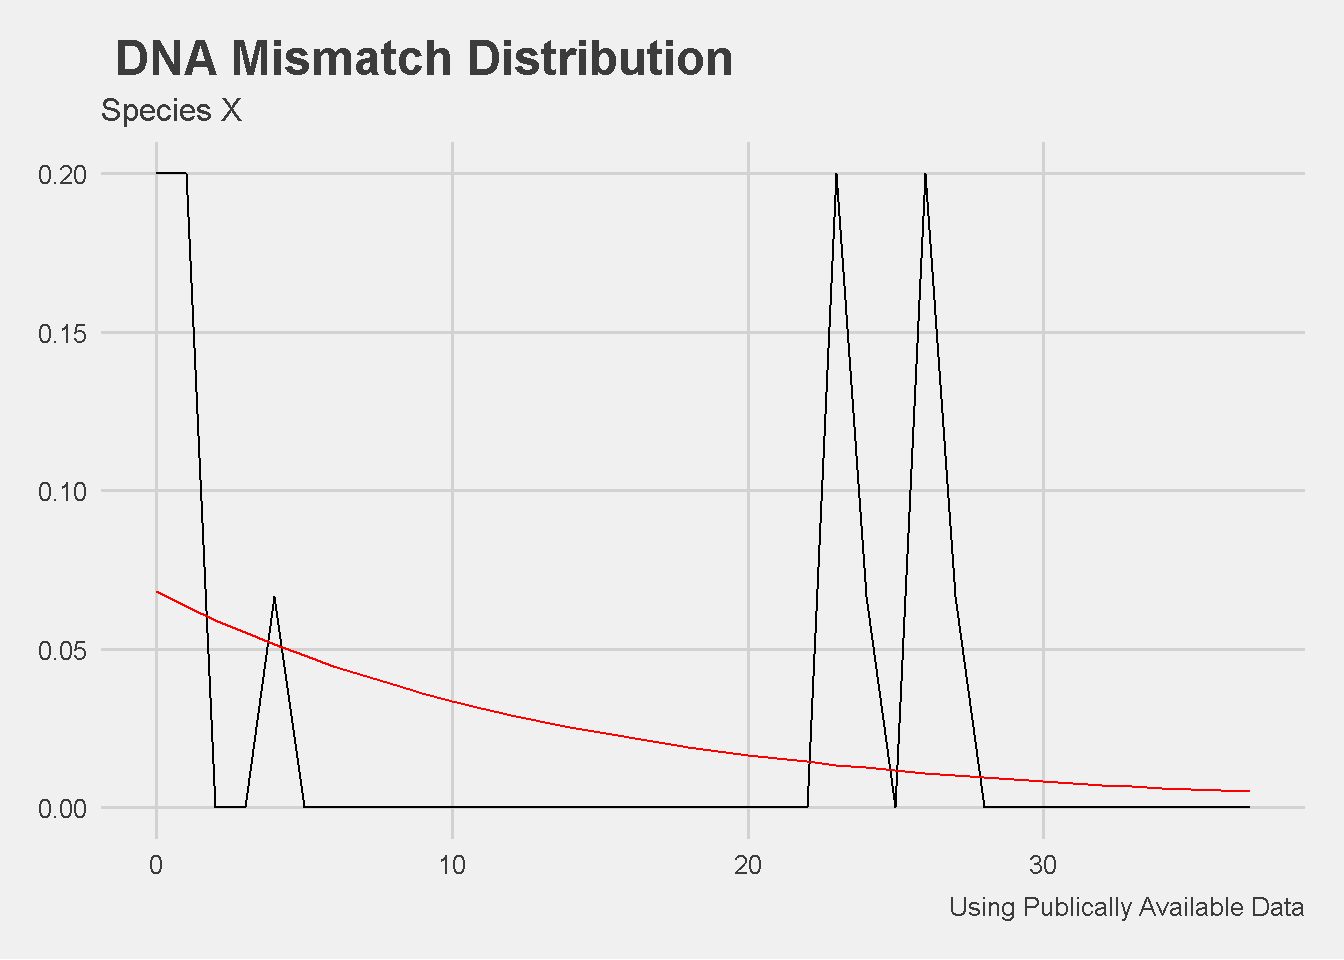
\includegraphics{mm_files/figure-latex/Plotting 1-1.pdf}

\subsubsection{\texorpdfstring{\href{sheading-2}{Saving Plot Using
\texttt{ggsave}}}{Saving Plot Using ggsave}}\label{saving-plot-using-ggsave}

\begin{Shaded}
\begin{Highlighting}[]
\KeywordTok{ggsave}\NormalTok{(}
  \DataTypeTok{filename =} \StringTok{"C:/Users/the_siff/Desktop/RR/DataScience/MyMM1.jpeg"}\NormalTok{,}
  \DataTypeTok{dpi =} \DecValTok{600}\NormalTok{, }\DataTypeTok{type =} \StringTok{"cairo"}\NormalTok{,}
  \DataTypeTok{height =} \FloatTok{2.71}\NormalTok{,}
  \DataTypeTok{width  =} \FloatTok{2.32}\NormalTok{,}
  \DataTypeTok{units =} \StringTok{"in"}
\NormalTok{)}
\end{Highlighting}
\end{Shaded}

A ggsave call will save the most recently produced ggplot2 plot within
your R console(use it carefully). The type argument is useful if you are
using R on windows due to anti-aliasing issues, which result in very
jagged lined plots. The dimensions arguments are optional and can be
left blank/default.

\subsection{\texorpdfstring{\href{sheading-2}{Method
2}}{Method 2}}\label{method-2}

\subsubsection{\texorpdfstring{\href{sheading-2}{Formatting Data into
the correct TIDY
format}}{Formatting Data into the correct TIDY format}}\label{formatting-data-into-the-correct-tidy-format}

\textbf{Frequency} column will take both sets of frequency calls and
\textbf{type} will contain expected and observed values

\begin{Shaded}
\begin{Highlighting}[]
\NormalTok{TidyMM <-}\StringTok{ }\KeywordTok{gather}\NormalTok{(MM,}
  \DataTypeTok{value =} \StringTok{"Frequency"}\NormalTok{,}
  \DataTypeTok{key =} \StringTok{"Type"}\NormalTok{,}
\NormalTok{  FreqObs, FreqExp}
\NormalTok{)}
\end{Highlighting}
\end{Shaded}

The gather function is native to tidyr, a component of the tidyverse
family. Frequency column will take both sets of frequency calls and type
will contain FreqExp and FreqObs values.

\subsubsection{\texorpdfstring{\href{sheading-2}{Comparing
Formats}}{Comparing Formats}}\label{comparing-formats}

\begin{Shaded}
\begin{Highlighting}[]
\KeywordTok{head}\NormalTok{(MM)}\OperatorTok\StringTok{ }\NormalTok{knitr}\OperatorTok{::}\KeywordTok{kable}\NormalTok{()     }\CommentTok{# Original}
\end{Highlighting}
\end{Shaded}

\begin{longtable}[]{@{}rrr@{}}
\toprule
Differences & FreqObs & FreqExp\tabularnewline
\midrule
\endhead
0 & 0.20000 & 0.06818\tabularnewline
1 & 0.20000 & 0.06353\tabularnewline
2 & 0.00000 & 0.05920\tabularnewline
3 & 0.00000 & 0.05516\tabularnewline
4 & 0.06667 & 0.05140\tabularnewline
5 & 0.00000 & 0.04790\tabularnewline
\bottomrule
\end{longtable}

\begin{Shaded}
\begin{Highlighting}[]
\KeywordTok{head}\NormalTok{(TidyMM) }\OperatorTok\StringTok{ }\NormalTok{knitr}\OperatorTok{::}\KeywordTok{kable}\NormalTok{() }\CommentTok{# Altered head}
\end{Highlighting}
\end{Shaded}

\begin{longtable}[]{@{}rlr@{}}
\toprule
Differences & Type & Frequency\tabularnewline
\midrule
\endhead
0 & FreqObs & 0.20000\tabularnewline
1 & FreqObs & 0.20000\tabularnewline
2 & FreqObs & 0.00000\tabularnewline
3 & FreqObs & 0.00000\tabularnewline
4 & FreqObs & 0.06667\tabularnewline
5 & FreqObs & 0.00000\tabularnewline
\bottomrule
\end{longtable}

\begin{Shaded}
\begin{Highlighting}[]
\KeywordTok{tail}\NormalTok{(TidyMM) }\OperatorTok\StringTok{ }\NormalTok{knitr}\OperatorTok{::}\KeywordTok{kable}\NormalTok{() }\CommentTok{# Altered tail}
\end{Highlighting}
\end{Shaded}

\begin{longtable}[]{@{}lrlr@{}}
\toprule
& Differences & Type & Frequency\tabularnewline
\midrule
\endhead
71 & 32 & FreqExp & 0.00712\tabularnewline
72 & 33 & FreqExp & 0.00663\tabularnewline
73 & 34 & FreqExp & 0.00618\tabularnewline
74 & 35 & FreqExp & 0.00576\tabularnewline
75 & 36 & FreqExp & 0.00537\tabularnewline
76 & 37 & FreqExp & 0.00500\tabularnewline
\bottomrule
\end{longtable}

\subsubsection{\texorpdfstring{\href{sheading-2}{Plotting Method
2}}{Plotting Method 2}}\label{plotting-method-2}

\begin{Shaded}
\begin{Highlighting}[]
\KeywordTok{ggplot}\NormalTok{(TidyMM, }\KeywordTok{aes}\NormalTok{(}
  \DataTypeTok{x =}\NormalTok{ Differences, }
  \DataTypeTok{y =}\NormalTok{ Frequency, }
  \DataTypeTok{linetype =}\NormalTok{ Type)) }\OperatorTok{+}
\StringTok{  }\KeywordTok{geom_line}\NormalTok{(}\DataTypeTok{show.legend =} \OtherTok{FALSE}\NormalTok{) }\OperatorTok{+}
\StringTok{  }\KeywordTok{theme_minimal}\NormalTok{() }\OperatorTok{+}
\StringTok{  }\KeywordTok{labs}\NormalTok{(}
    \DataTypeTok{subtitle =} \StringTok{"Species X"}\NormalTok{,}
    \DataTypeTok{title =} \StringTok{" DNA Mismatch Distribution "}\NormalTok{,}
    \DataTypeTok{caption =} \StringTok{"Using Publically Available Data"}\NormalTok{,}
    \DataTypeTok{x =} \StringTok{"Differences"}\NormalTok{,}
    \DataTypeTok{y =} \StringTok{"Frequency Observed"}\NormalTok{)}\OperatorTok{+}
\StringTok{  }\KeywordTok{theme_fivethirtyeight}\NormalTok{()}
\end{Highlighting}
\end{Shaded}

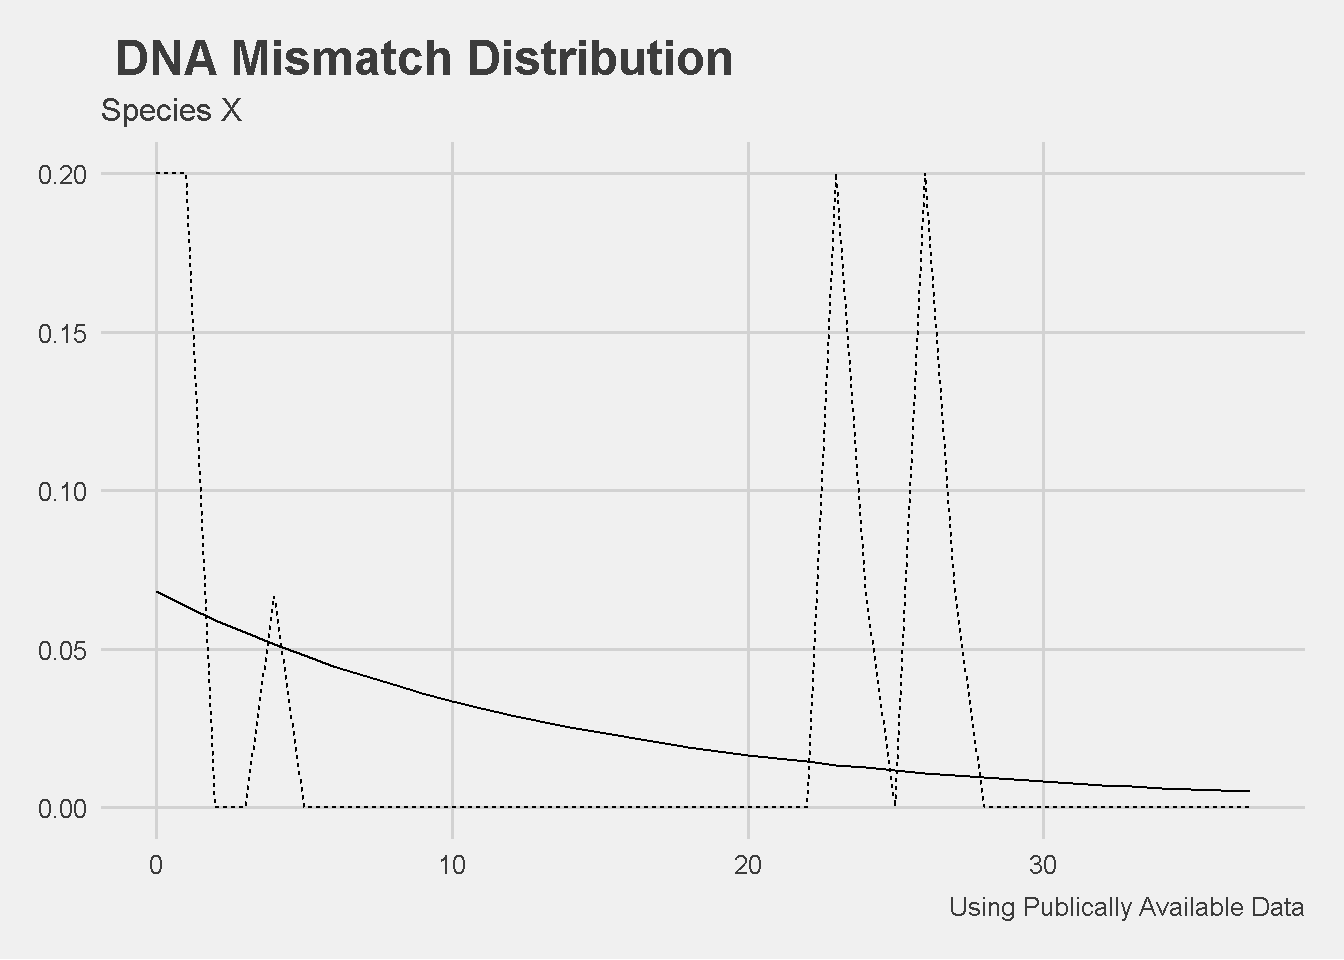
\includegraphics{mm_files/figure-latex/Plotting Data 2-1.pdf}

\subsubsection{\texorpdfstring{\href{sheading-2}{Saving Plot Using
\texttt{ggsave}}}{Saving Plot Using ggsave}}\label{saving-plot-using-ggsave-1}

\begin{Shaded}
\begin{Highlighting}[]
\KeywordTok{ggsave}\NormalTok{(}
  \DataTypeTok{filename =} \StringTok{"C:/Users/the_siff/Desktop/RR/DataScience/MyMM2.jpeg"}\NormalTok{,}
  \DataTypeTok{dpi =} \DecValTok{600}\NormalTok{, }\DataTypeTok{type =} \StringTok{"cairo"}\NormalTok{,}
  \DataTypeTok{height =} \FloatTok{2.71}\NormalTok{,}
  \DataTypeTok{width  =} \FloatTok{2.32}\NormalTok{,}
  \DataTypeTok{units =} \StringTok{"in"}
\NormalTok{)}
\end{Highlighting}
\end{Shaded}


\end{document}
